\section{Introduction}

You've probably seen that a pencil in a glass of water looks ``bent.'' If you 
haven't, before reading any further, take a glass of water and a pencil, fill 
the glass half-way with water and place the pencil in.  Look down from above 
the water's surface; the pencil will appear to be bent at the water's surface.
It isn't really the pencil that's bent, the light rays coming from the pencil
are bent at the air-water interface with the result that the pencil looks bent.
This phenomenon of light rays being bent at the interface between two media, 
such as air and water, is called the {\it refraction of light}.  We'll study 
several aspects and applications of it in this lab.  

We'll examine the physical law, Snell's law, that describes the geometry of 
refraction ({\it i.e.}, how ``bent'' the pencil appears). We'll see that 
refraction occurs because light travels at different speeds in different 
media; we'll learn how to quantify this by defining the {\it index of 
refraction} of a medium.  We'll also see that, for a given medium, there is a 
certain angle of incidence, called the {\it critical angle}, for which all of 
the incident light is reflected.  This is called {\it total internal 
reflection} and it has important applications, which include the field of 
fiber optics. 

\section{Theory}

\subsection{References}

The nature of light and refraction is covered in Serway, Chapter~35 (The 
Nature of Light and the Laws of Geometric Optics).  Much of what we'll
discuss will go a bit easier if you read the very short Section~35.1 (The 
Nature of Light), which describes the properties of light. Also 
useful are Sections~35.4 (Reflection and Refraction),   
35.6~(Huygen's Principle), and~35.7 (Total Internal Reflection), 
which discuss Snell's law and total internal reflection.  


\subsection{Index of Refraction}

At some point in your career as a student, someone will tell you that the 
speed of light in a vacuum is a constant, denoted by the letter $c$, whose 
value is $c=2.997~924~58 \cdot 10^8$~m/s.  This statement of the constancy of 
the speed of light has been verified by experiment and forms the basis for
Albert Einstein's Theory of Relativity.  We're not going to discuss relativity
here, we only want to make the point that $c$ refers to light in vacuum, that
is, in a box, let's say, in which there is no air or anything else.  If the
light is traveling through a medium, perhaps a glass slab, or even the Earth's
atmosphere, it will interact with the medium.  Some of the light will ``bounce 
off'' of the atoms and molecules that make up the medium and, as a result,
light will (almost) always travel slower through a medium.  How much slower 
depends on the properties of the medium: its chemical composition, its density,
temperature, etc.  Also, the speed depends on the wavelength of light, a 
phenomenon called {\it dispersion}.  We won't have the chance to explore this
important and very interesting phenomenon, which is responsible for rainbows 
and the spectrum of colors emerging from prisms, but you are encouraged to read
about it in Serway, Section 35.5 (Dispersion and Prisms), p.\ 994.

We can always express the velocity of light in a medium in terms of the vacuum
value $c$.  A convenient way of doing so is to define the {\it index of 
refraction}, denoted by $n$, as the ratio of $c$ to $v$, the velocity of light
in the medium, 
$$ n=\frac{c}{v}. $$ 
It is easy to see that $n$ is a dimensionless number and, since $v$ will be 
less than $c$ for most materials, $n$ is greater than one.  Since $v$ depends 
on the wavelength of the light, so does the index of refraction.  We'll try to
always report a value of $n$ for a specific wavelength.  If the index of 
refraction doesn't vary too much over a range of wavelengths, typically the 
visible band, we might quote a single value (of an appropriate number of 
significant figures) that is good over that range.

What are some typical values of the index of refraction?  Air has an index of
refraction which is very nearly equal to one.  At 15$^\circ$C, 
$n_{\mbox{air}}$ varies from $1.000~325~6$ (at a wavelength of 200~nm) to
$1.000~273~6$   (at 1000~nm) over the visible band. We'll be using red He-Ne 
laser light in the lab, with wavelength 632.8~nm, for which 
$n_{\mbox{air}}=1.000~276~0$.  To a high degree of accuracy, we may take
$n_{\mbox{air}}\sim 1$.  At 25$^\circ$C, water has an index of refraction
that varies from 1.452 (at 200~nm) to 1.322 (at 1000~nm). Glass is rather 
difficult to state a precise index of refraction for, chiefly because there
are many different types and ways of making glass.  In the lab we'll be using
Plexiglas, which has a refractive index of roughly 1.49 and crown glass, which
has $n\sim 1.52$.  

Some terminology that is commonly used is to refer to media as being fast or
slow.  Fast media have small indices of refraction, while slow ones have
larger indices of refraction.  It should be clear that these are relative 
terms. For example, water is a fast medium compared to 
glass, but is slow compared to air. 


\subsection{Refraction at a Boundary - Snell's Law}

We will consider a light ray which crosses the boundary between two media of 
indices of refraction $n_1$ and $n_2$, illustrated in 
Figure~\ref{fig:opt:interface}.
\begin{figure}[htb]
\centering 
\epsfxsize=6cm 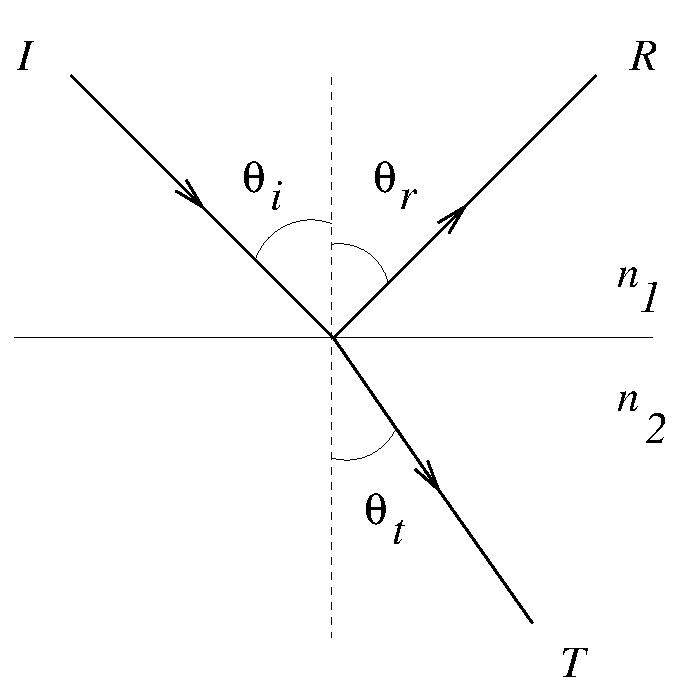
\includegraphics[scale=0.6]{8_refraction/interface.eps}
\caption{A ray of light incident on the interface between two media.}
\label{fig:opt:interface}
\end{figure}
The primary ray $I$ is called the {\it incident ray}, $R$ is called the 
{\it reflected ray}, and $T$ is the {\it transmitted}, or {\it refracted ray}.
All angles are defined with respect to the {\it normal} to the surface. We 
would like to know how the angle of reflection, $\theta_r$, and the angle
of refraction, $\theta_t$, depend on the angle of incidence, $\theta_i$, and
$n_1$ and $n_2$.

We'll examine this by considering two parallel rays and using the somewhat 
obvious fact that points along the rays will travel at the same velocity in a 
given medium.  Consider Figure~\ref{fig:opt:parallelpts},
\begin{figure}[htb]
\centering 
\epsfxsize=6cm 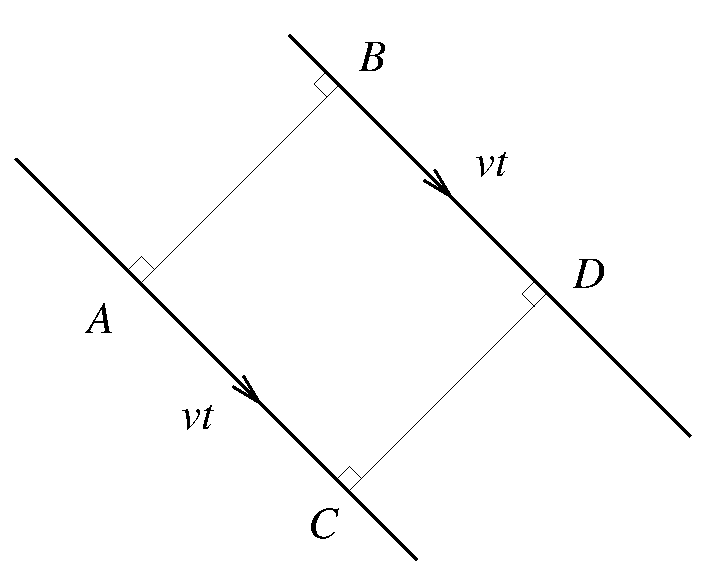
\includegraphics[scale=0.6]{8_refraction/parallelpts.eps}
\caption{Corresponding points correspond to equal times.}
\label{fig:opt:parallelpts}
\end{figure}
which illustrates two parallel rays, where the points $A$ and $B$ correspond
to parallel points along the rays, since the line segment $\overline{AB}$ is 
perpendicular to both of the rays. Similarly $C$ and $D$ are parallel points 
and therefore the distances $\overline{AC}$ and $\overline{BD}$ are equal.
If it takes a time $t$ for the light to traverse the distance from $A$ to $C$, 
then we can write $\overline{AC}=vt$. Since $\overline{AC}=\overline{BD}$, we 
have $\overline{BD}=vt$ as well, so that the time taken to go from $B$ to $D$
is also $t$. We can say that corresponding points along two parallel light 
beams correspond to equal times.

Let's apply this to an interface; for simplicity we'll consider the reflected
and refracted rays separately.  First, the reflected rays are drawn in 
Figure~\ref{fig:opt:reflected}.
\begin{figure}[htb]
\centering 
\epsfxsize=10cm 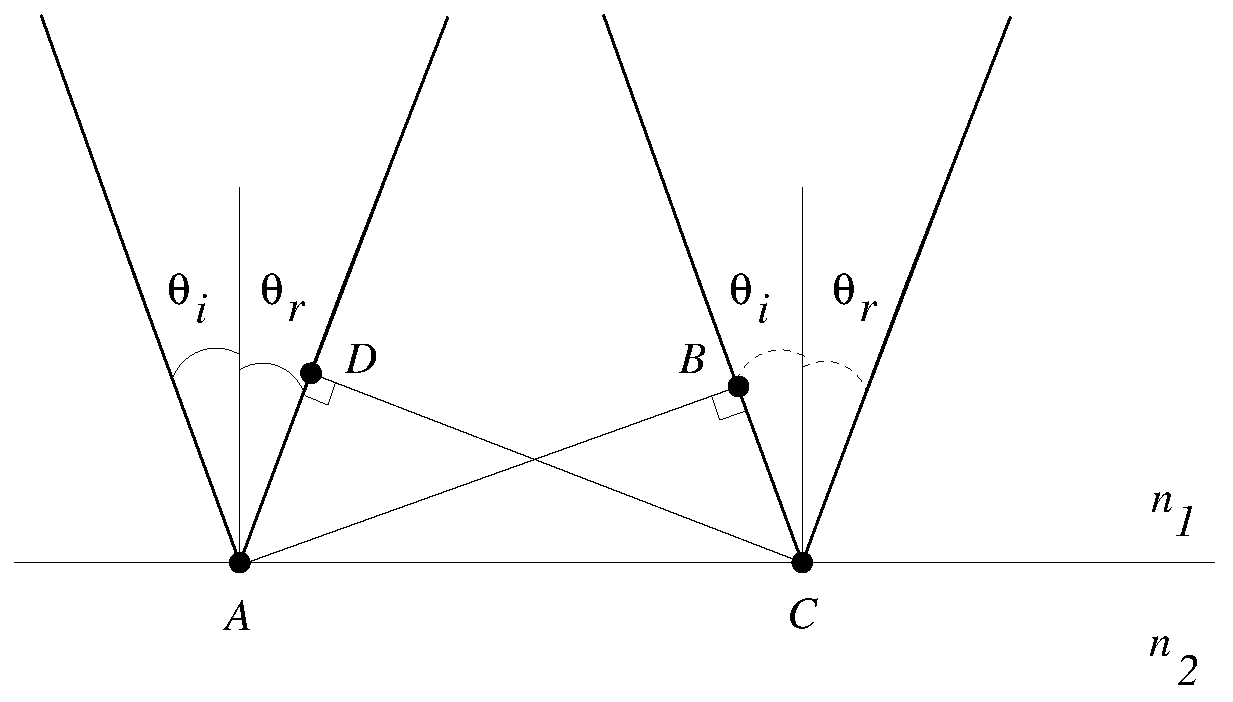
\includegraphics[scale=0.6]{8_refraction/reflected.eps}
\caption{The incident and reflected rays at an interface.}
\label{fig:opt:reflected}
\end{figure}
Simple geometry tells us that the angles $\angle BAC =\theta_i$ and 
$\angle ACD =\theta_r$. If we take $\overline{BC}=v_1 t$ then, since 
$\overline{BC}=\overline{AC}\sin\theta_i$,we have
$$ \overline{AC}\sin\theta_i = v_1 t. $$ 
By applying the equal time rule to points $A$ and $B$ and then $C$ and $D$, we
have $\overline{AD}=\overline{BC}$, so that 
$$ \overline{AC}\sin\theta_r = \overline{AD} = v_1 t. $$ 
We can then take the ratio
$$ \frac{\overline{AC}\sin\theta_r}{\overline{AC}\sin\theta_i} 
=\frac{v_1 t}{v_1 t}, $$
so that we find
$$ \sin\theta_r=\sin\theta_i, $$
or simply
$$ \theta_r=\theta_i. $$
This is a famous result, {\it the angle of reflection is equal to the angle of
incidence}.

We can now look at the refracted rays, in Figure~\ref{fig:opt:refracted}.
\begin{figure}[htb]
\centering 
\epsfxsize=10cm 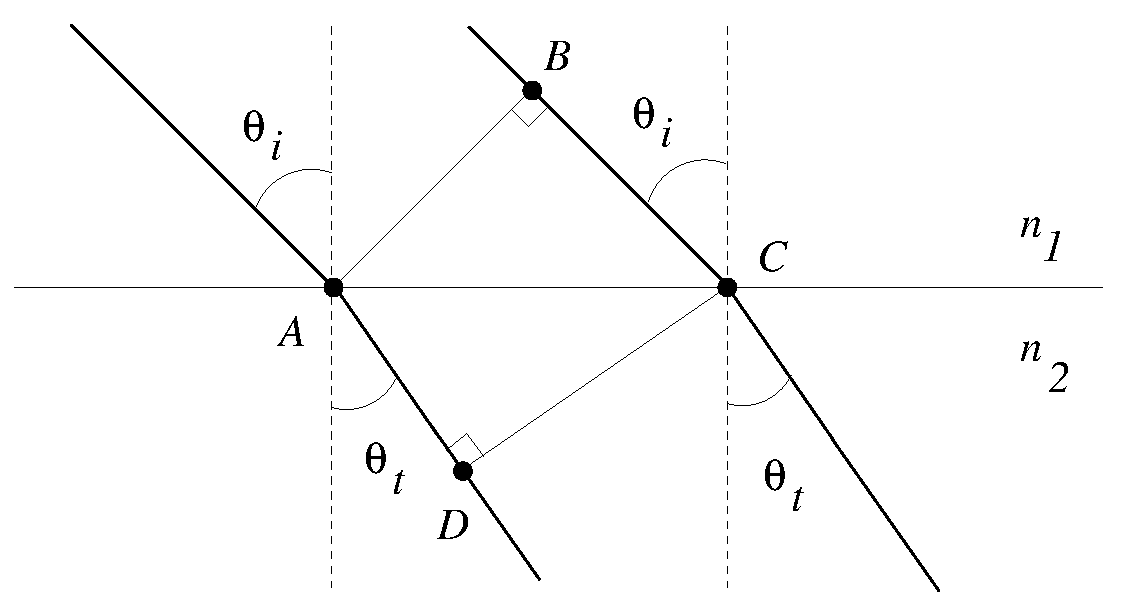
\includegraphics[scale=0.6]{8_refraction/refracted.eps}
\caption{The incident and refracted rays at an interface.}
\label{fig:opt:refracted}
\end{figure}
Here we have $\angle BAC =\theta_i$ and $\angle ACD =\theta_t$ and can write
$\overline{BC}=v_1 t$ and $\overline{AD}=v_2 t$ by the equal time rule. Then
\begin{eqnarray*}
\overline{AC}\sin\theta_i &=& \overline{BC}=v_1 t \nonumber \\
\overline{AC}\sin\theta_t &=& \overline{AD}=v_2 t, \\
\end{eqnarray*}
which tells us that
$$ \frac{\sin\theta_i}{\sin\theta_t} =\frac{v_1}{v_2} =\frac{c/n_1}{c/n_2}, $$
which we write as 
\begin{equation}
\fbox{$ \displaystyle n_1\sin\theta_i=n_2\sin\theta_t,$} \label{eq:opt:snell}
\end{equation}
which is known as Snell's law.   

To summarize our results, we look back at Figure~\ref{fig:opt:interface}.
If the light is incident at an angle $\theta_i$, then we know that the 
reflected angle is equal to the incident angle, $\theta_r=\theta_i$, while
the refracted angle, $\theta_t$, may be found from Snell's 
law~(\ref{eq:opt:snell}).  We also note that when $n_2>n_1$, that is, when we
are passing from a fast medium to a slow medium, Snell's law tells us that the 
angle of refraction will be smaller than the angle of incidence. When moving 
from a slow medium to a fast medium, we will have $\theta_t >\theta_i$.

Let's consider a light ray incident on a glass slab (index $n$) in air 
($n_{\mbox{air}}\sim 1$), illustrated in Figure~\ref{fig:opt:slab}.
\begin{figure}[htb]
\centering 
\epsfxsize=10cm 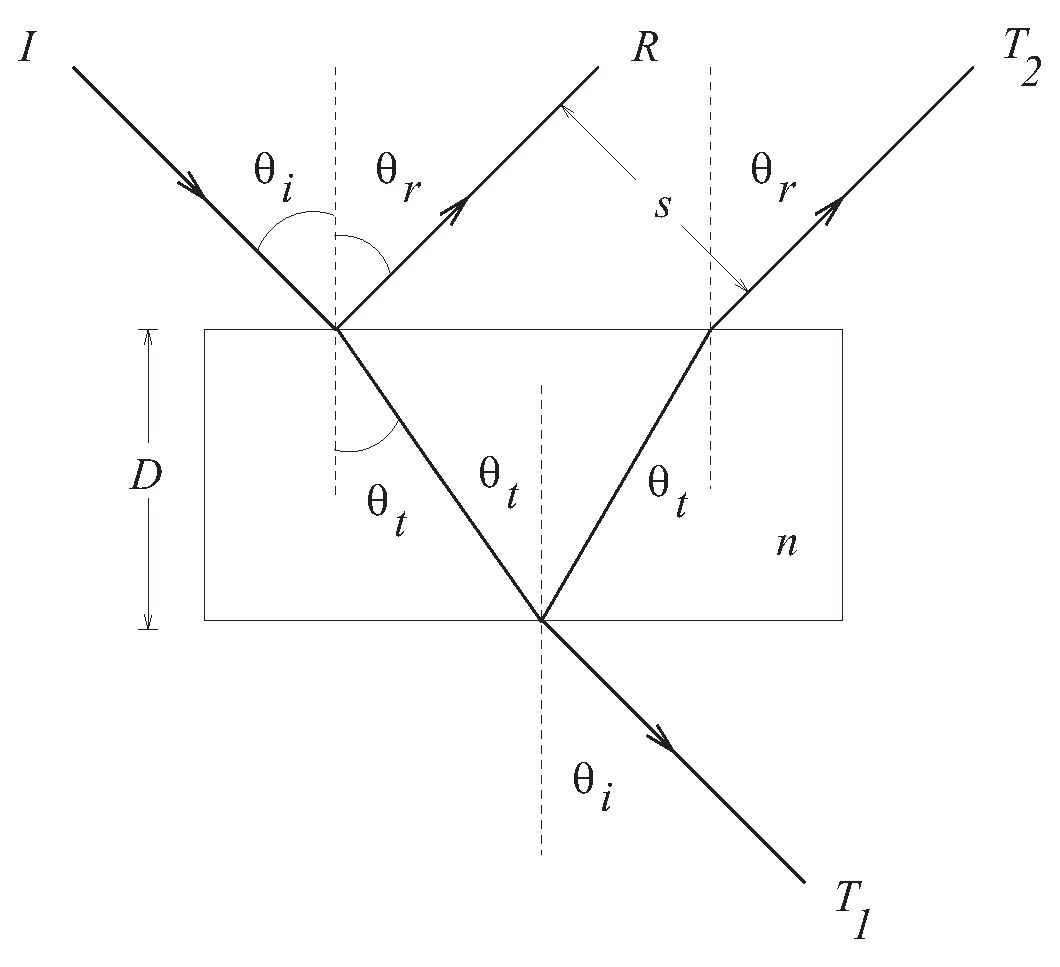
\includegraphics[scale=0.6]{8_refraction/slab.eps}
\caption{The glass slab.}
\label{fig:opt:slab}
\end{figure}
If the faces of the slab are perfectly parallel, then the reflected ray $R$ 
and the ray $T_2$ will be parallel. We can determine the dependence of the 
distance between them, s, on the incident angle and the width, $D$, by 
using Snell's law and a bit of trigonometry;  the result can be determined 
without considering velocities or times. The student is encouraged to show as 
an exercise that
\begin{equation}
\fbox{$ \displaystyle s =\frac{2D\sin\theta_i\cos\theta_i}{\sqrt{n^2-\sin^2\theta_i}}. $}
\label{eq:opt:slab}
\end{equation}

\subsection{Total Internal Reflection}
\label{sec:opt:totintref}

Let's examine the possibility that, for a certain angle of incidence, the 
refracted angle, $\theta_t=90^\circ$, as shown in 
Figure~\ref{fig:opt:totintref}.
\begin{figure}[htb]
\centering 
\epsfxsize=6cm 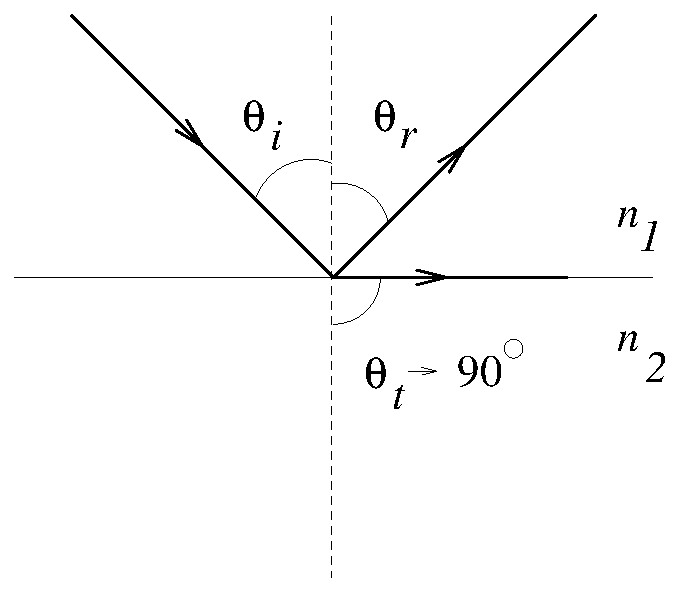
\includegraphics[scale=0.6]{8_refraction/totintref.eps}
\caption{Total internal reflection occurs when the refracted ray cannot exit
the primary medium.}
\label{fig:opt:totintref}
\end{figure}
In other words, there is no refracted ray, since it does not exit medium 1.
All of the incident light is reflected by the interface and none of it is
transmitted. How can this happen?

Let's try to answer this by first noting that for $\theta_t=90^\circ$,
$\sin\theta_t=1$, so that Snell's law reads
\begin{equation}
\sin\theta_i=\frac{n_2}{n_1},  \label{eq:opt:condtir}
\end{equation}
or 
$$
\fbox{$ \displaystyle \theta_i=\sin^{-1}\left(\frac{n_2}{n_1}\right). $} 
$$
Remember that $n_1$ and $n_2$ refer to the first medium
and the second medium respectively.  
Now it is an extremely familiar property of the sine function that its 
magnitude is always less than or equal to one,
\begin{equation}
|\sin\theta| \leq 1 ~\mbox{for all}~\theta, 
~~~\sin\theta=1 ~\mbox{only for}~\theta=90^\circ.  \label{eq:opt:sinbound}
\end{equation}
We can consider the case that medium 1 is faster than medium 2, or $n_2>n_1$,
then equation~(\ref{eq:opt:condtir}) requires that $\theta_i$ satisfy
$$
\sin\theta_i >1.
$$ 
This is impossible due to the fundamental property~(\ref{eq:opt:sinbound}),
so we conclude that there is no incident angle for which $\theta_t=90^\circ$,
when $n_2>n_1$.
 
If, instead, medium 2 is faster than medium 1, $n_2<n_1$, then we have
$$
\sin\theta_i <1.
$$ 
Therefore, there is {\it some} incident angle, we'll call it the critical 
angle, $\theta_{\mbox{crit}}$, satisfying
\begin{equation}
\fbox{$ \displaystyle \theta_{\mbox{crit}}=\sin^{-1}\left(\frac{n_2}{n_1}\right), $}
\label{eq:opt:totintref}
\end{equation}  
for which there will be no refracted ray. Note that
we have switched our point of view.  We are now using the larger index
of refraction as $n_1$ and the smaller as $n_2$.
As an exercise the student should
come up with an argument for why there will also be no refracted ray if the 
angle of incidence is {\it greater} than $\theta_{\mbox{crit}}$. This 
phenomenon is called {\it total internal reflection}: {\it when passing from a 
slow medium into a faster medium, there is a critical angle of incidence, such 
that for incident angles greater than or equal to the critical angle, all of 
the light will be reflected from the interface}.

Total internal reflection has one application in the field of fiber optics.
There, a glass fiber is used to carry a light beam, as in 
Figure~\ref{fig:opt:fiber}.
\begin{figure}[htb]
\centering 
\epsfxsize=12cm 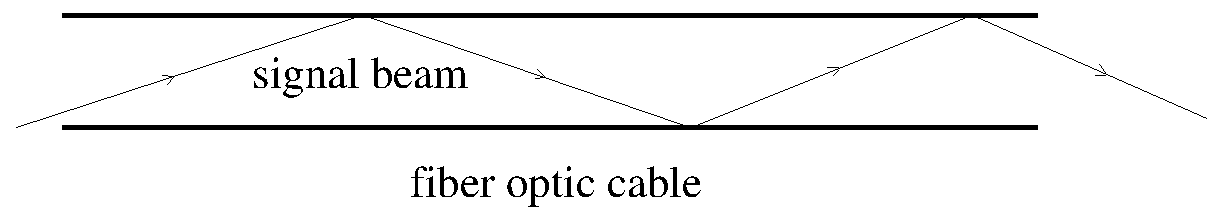
\includegraphics[scale=0.6]{8_refraction/fibopt.eps}
\caption{A depiction of a fiber optic cable.}
\label{fig:opt:fiber}
\end{figure}
The angle of incidence for each ``bounce'' off of the walls of the cable is
kept greater than the critical angle determined from Snell's law. As a result,
the signal is kept almost completely intact over its transit through the cable,
which can be hundreds of miles long.  Clearly this is an efficient means of
transmitting information encoded into a light signal. Serway provides a nice
discussion of fiber optics in the essay on page 1009.


\section{Apparatus}

For our refraction experiments we will be using a He-Ne laser.  This produces
red light with a wavelength of 632.8~nm.  The laser produces an intense
beam of light that is difficult to duplicate with a white light source.  Using
such an intense beam does not come without a price; we must be particularly 
cautious when using the laser.


\begin{center}
{\bf Laser Safety Guidelines:}
\end{center}

\begin{itemize}

\item Avoid looking directly into the laser beam or its reflections.  The laser
light is intense enough to burn the retina and permanently impair vision if 
it comes into direct contact with the eye. 

\item A ``dish'' with a steel rim will be provided for containing the laser 
beam during use. The laser should not be turned on unless it is safely pointed 
inside the dish.

\item Do not point the laser across the room or into the air; doing so will 
endanger everyone else in the room.

\item Do not point the laser through the lenses.

\end{itemize}
We'll use a Plexiglas slab with an index of refraction of about 1.49 to 
examine Snell's law. To investigate total internal reflection, we'll use a
prism made of crown glass, which has an index of refraction of about 1.52. 


\vfill
\pagebreak
$$
$$
\vfill
\clearpage
\newpage

%  Label worksheets by \thechapter.W
\renewcommand{\thesection}{\thechapter.W}

\section{Refraction Worksheet}
{\bf \Large Name:}~ \rule{5cm}{.1mm}~~~~~~~
{\bf \Large Day/Time:}~\rule{3cm}{.1mm}\\
{\bf \Large Partner's Name:}~\rule{6cm}{.1mm}\\
\subsection{In-Lab Procedure}

\subsubsection{Ray Tracing}
\label{sec:opt:raytrace}

We are using lasers for our refraction studies so that we have clear, well 
defined beams of light, such as those we've been drawing in our figures. 
We'll use our experimental set-up to trace these beams and the objects we're 
using to refract the light onto a sheet of paper.  This will give us a picture
of what was going on, called a {\it ray tracing}, and will make it easy to 
measure angles and distances, so that we can tell if Snell's law is really 
valid. \\

\noindent What is a ray tracing? It is a projection of the light rays passing through 
our apparatus onto a sheet of paper. How do we make a ray tracing?  First of 
all, we place the refracting object, say a Plexiglas slab, on top of a large 
sheet of computer paper that we've taped to the bottom of the laser dish.  The 
set-up and several of the light rays are shown in 
Figure~\ref{fig:opt:slabproc}a. 
\begin{figure}[htb]
\centering 
\epsfxsize=13cm 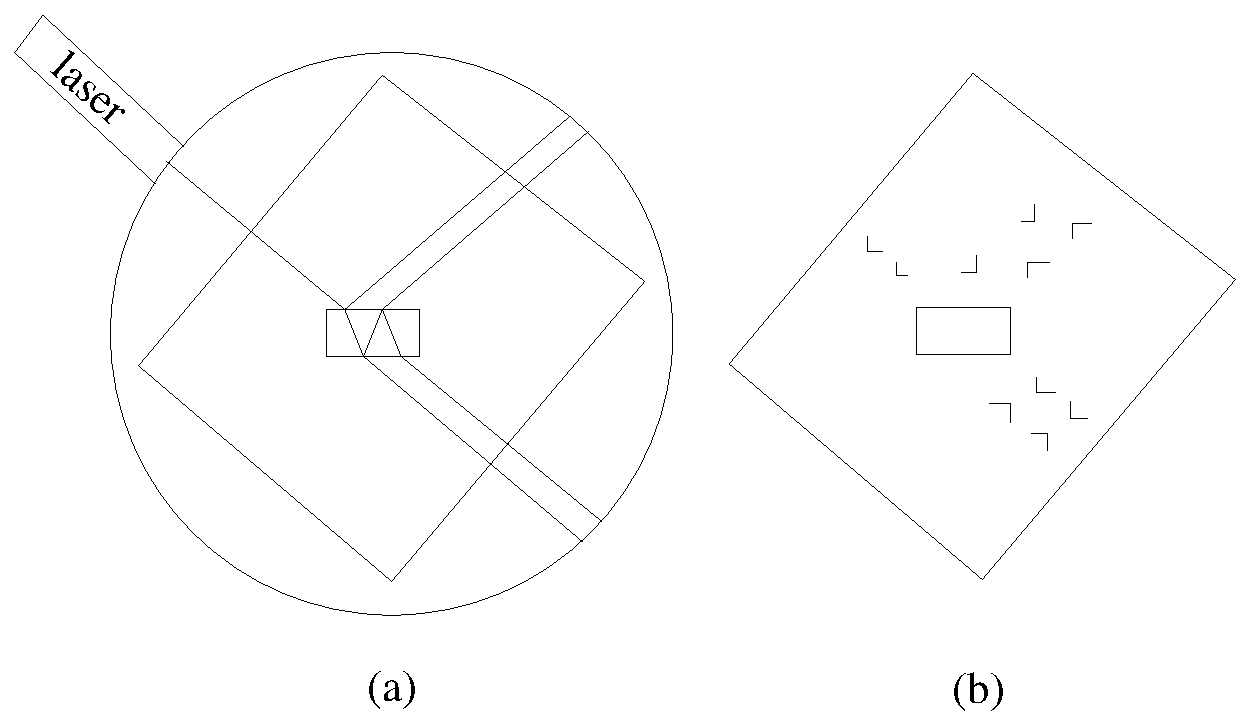
\includegraphics[scale=0.6]{8_refraction/slabproc.eps}
\caption{The set-up for ray tracing with a Plexiglas slab.}
\label{fig:opt:slabproc}
\end{figure}
We then trace each ray individually.  Using a corner of a glass block, we'll 
block off the beam, as shown in Figure~\ref{fig:opt:raytrace}. Be careful that
you avoid looking directly into the reflection of the beam from the block.
\begin{figure}[htb]
\centering 
\epsfxsize=10cm 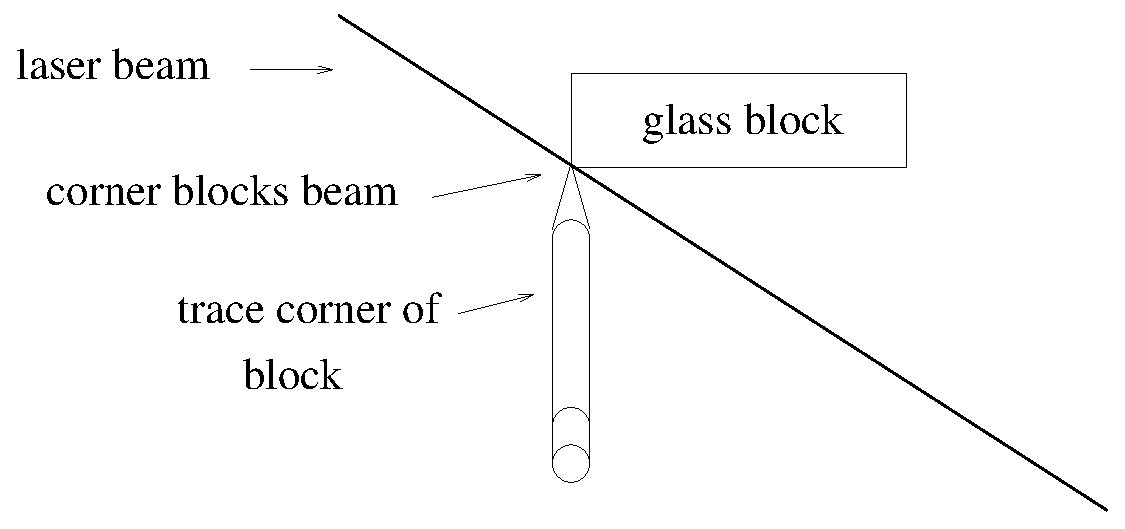
\includegraphics[scale=0.6]{8_refraction/raytrace.eps}
\caption{Ray tracing is done by blocking the beam and then marking off the 
corner of the block.}
\label{fig:opt:raytrace}
\end{figure}
The laser beam has a finite width, so that we can partially block off the beam,
if we position the glass block properly. We'll block the beam so that the 
glass block is approximately at the {\it center} of the beam, then we'll make 
two pencil marks at the corner of the block. What we've done is taken a point 
on the beam, which is above the paper, and projected it down to a point on the 
paper.  If we move to another section of the beam and repeat this procedure, 
we'll have two points on the beam marked on the paper.  By drawing a line 
through these two points, we can reproduce the path that the beam took. \\

\noindent Figure~\ref{fig:opt:slabproc}b illustrates how a raytracing of all the beams
in  Figure~\ref{fig:opt:slabproc}a will appear.  All of the rays have been 
marked in two places by the procedure outlined; the glass slab has also been
traced.  By connecting the corresponding points with straight lines, we can
reproduce all of the rays found outside the slab in 
Figure~\ref{fig:opt:slabproc}a. By connecting the corresponding points where 
these rays intersect with the outline of the slab, we can draw the interior 
rays.


\subsubsection{Snell's Law and a Glass Slab}

Set up the laser and Plexiglas slab exactly as shown in 
Figure~\ref{fig:opt:slabproc}a.  Perform the ray tracing as outlined in 
$\S$~\ref{sec:opt:raytrace}. {\bf Be sure to outline the Plexiglas block}. 
It will 
probably help you to label the marks you make during the ray tracing as the 
incident ray, the first reflected ray, etc. When you've traced all of the rays 
that you can, pick the paper up and connect the corresponding points with a 
straight edge.  Connect the intersecting points at the slab outline to 
visualize the internal rays. Before continuing to the next procedure,
look at your tracing and answer the following rhetorical questions.
Does the resulting tracing appear as you expected 
it to?  Do the sides of the slab appear to be parallel? How do the rays that 
you've traced allow you to determine this?  \\
 

\subsubsection{Total Internal Reflection}

Place a new sheet of computer paper in the laser dish and place the prism on it.
Aim the laser through one of the short sides of 
the prism, shown in Figure~\ref{fig:opt:tirproc}a.
\begin{figure}[htb]
\centering 
\epsfxsize=14cm 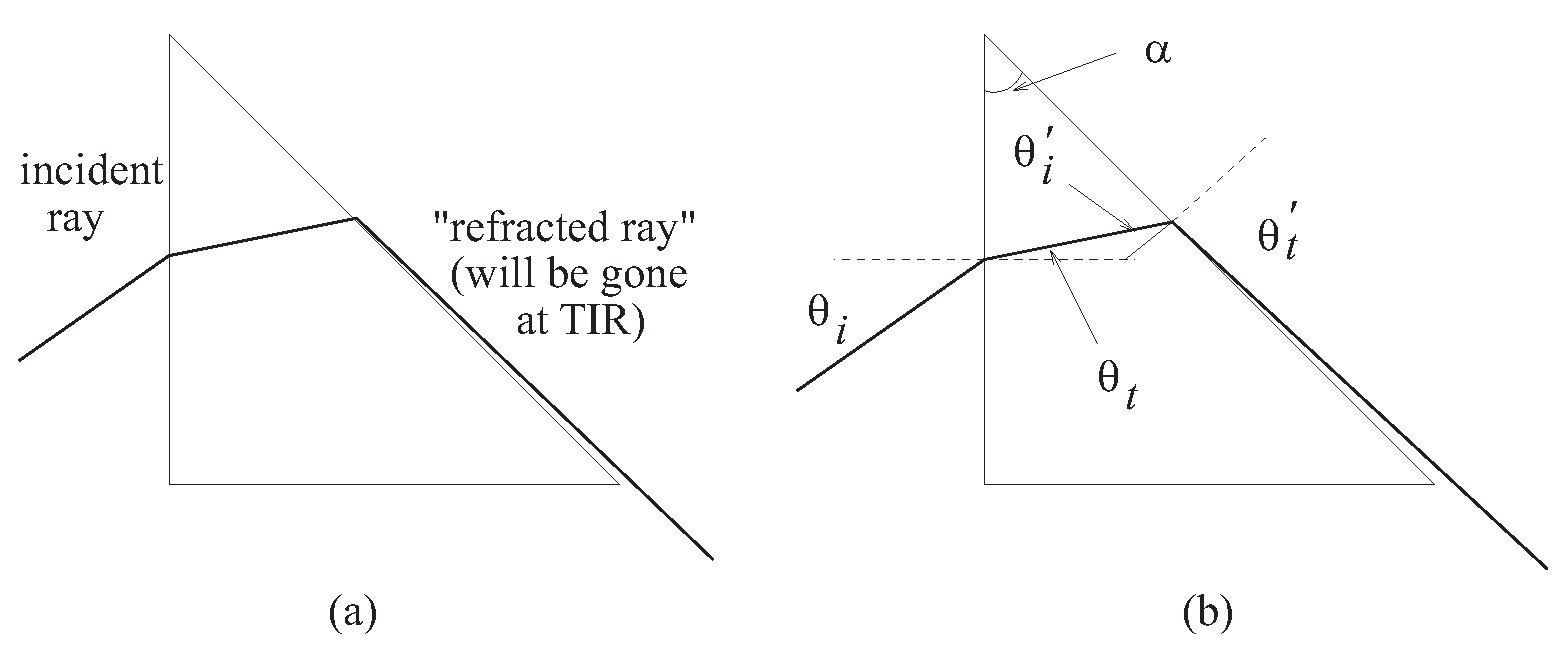
\includegraphics[scale=0.6]{8_refraction/tirproc.eps}
\caption{Total internal reflection with the prism.}
\label{fig:opt:tirproc}
\end{figure}
Start with an incident angle ($\theta_i$ in Figure~\ref{fig:opt:tirproc}b)
of approximately $30^\circ$ and decrease the incident angle, while keeping an
eye on the ray labeled ``refracted ray'' in Figure~\ref{fig:opt:tirproc}b.  
Is there an incident angle $\theta_i$ for which the refracted ray disappears?
Locate the critical angle; when you find it, leave the prism in place and 
{\bf trace the outline of the prism and the incident ray}. \\

\subsection{Pre-Classroom Check List}
\noindent $\bigcirc$ \hspace*{1cm} Ray tracing of slab and at least four
rays per person \\
$\bigcirc$ \hspace*{1cm} Ray tracing of prism and incident ray per person
 


\subsection{In-Classroom Calculations \& Analysis}
\subsubsection{Snell's law and a Glass Slab}

At the vertex where the incident ray, the first reflected ray and the first 
interior (refracted) ray meet, use a protractor to measure
the angle of incidence $\theta _i,$ the angle of reflection $\theta _r,$
and the angle of refraction $\theta _t.$ Record these values 
(with uncertainties) below.  To account for any errors introduced in the
ray tracing procedure, take approximately $2^\circ$ uncertainty in all of your 
angle measurements. \\

\begin{center}
$\theta _i=$~ \rule{3cm}{.1mm} ~~~~
$\theta _r=$~ \rule{3cm}{.1mm}

$\theta _t=$~ \rule{3cm}{.1mm}
\end{center} 
\vspace*{.5cm}
 
\noindent Does $\theta_r=\theta_i$ within uncertainty? \\
\vspace*{2cm} \\
\noindent Assuming that the index of refraction of air, $n_{air}$, 
is 1, use Snell's Law to determine
a value for the index of refraction of the Plexiglas slab, $n_{slab},$ 
{\it with
uncertainty.} Showing your work, record this value below. \\
\vfill
\begin{center}
$n_{slab}=$~ \rule{3cm}{.1mm} 
\end{center}
\newpage
\noindent  How does this compare with the expected value
$n\sim 1.49$? \\
\vspace*{1cm}

\noindent Now, referring to Figure~\ref{fig:opt:slab}, measure $D$ of 
the Plexiglas slab from your outline. \\
\begin{center}
$D=$~ \rule{3cm}{.1mm} ~~~~
\end{center}
\noindent  Given that the rays you use to {\it measure} $s$
may not be perfectly parallel (you'll have to look at your sketch to find out),
determine a typical value of $s$ from your sketch and calculate an uncertainty
for it that takes into account any deviations of the rays from being parallel.
This isn't as hard as it may sound, just use common sense to get a ball-park
figure and let your uncertainty account for the arbitrariness in doing so. \\
\vspace*{2cm} \\
\begin{center}
$s_{meas}=$~ \rule{3cm}{.1mm}
\end{center}

\noindent
Calculate the value predicted by equation~(\ref{eq:opt:slab}) for
the distance between the primary and secondary reflected rays,
$s_{calc},$ {\it with uncertainty.}  Make sure you use your value of
$n_{slab}$ for $n$ in this equation.  Record the calculated value
below. {\bf SHOW WORK}. \\
\vspace*{7cm} \\
\begin{center}
$s_{calc}=$~ \rule{3cm}{.1mm}
\end{center}


\subsubsection{Total Internal Reflection}


As is illustrated in Figure~\ref{fig:opt:tirproc}b, $\theta_i$ is 
{\it not} the critical angle we were referring to in our discussion of total 
internal reflection in $\S$~\ref{sec:opt:totintref}. Since total internal 
reflection is occurring at the {\it second} glass to air interface, the 
critical angle corresponds to the incident angle $\theta_i^\prime$ in  
Figure~\ref{fig:opt:tirproc}b.  How can we determine $\theta_i^\prime$?  
Measure the prism angle, $\alpha$, and $\theta_i$.  \\
\begin{center}
$\alpha = $~ \rule{3cm}{.1mm} ~~~~
$\theta _i=$~ \rule{3cm}{.1mm}
\end{center}
\vspace*{.5cm}

\noindent From Snell's law, we find at the first interface that
$$
\theta_t = \sin^{-1}\left( \frac{1}{n} \sin\theta_i \right),
$$
where the index of refraction of the prism, $n\sim 1.52$.  By simple
geometry, we can calculate $\theta_i^\prime$ from
$$
\theta_i^\prime = \alpha-\theta_t.
$$
First use this to calculate $\theta_t$ {\it with uncertainty}. {\bf SHOW WORK}.
\\
\vspace*{2cm} \\
\begin{center}
$\theta _t=$~ \rule{3cm}{.1mm}
\end{center} 

\noindent
Calculate a value for $\theta '_i$ {\it with uncertainty.} 
Also, use equation~\ref{eq:opt:totintref} to calculate the critical angle of
incidence for total internal reflection in crown glass, $\theta _{crit}.$
(Again, use $n \sim 1.52$ for the index of refraction of the prism.) Record
these values below.  Use the space above the recorded values to {\bf show your
work}. \\
\vspace*{3.5cm} \\
\begin{center}
$\theta '_i=$~ \rule{3cm}{.1mm} ~~~~ 
$\theta _{crit}=$~ \rule{3cm}{.1mm}
\end{center} 


\subsection{In-Classroom Discussion}
\subsubsection{Snell's Law and a Glass Slab}
\noindent
Do the sides of the Plexiglas slab appear to be parallel?
\vspace*{.3cm}

\noindent
Explain how the rays that you've traced allow you to determine this.
\vspace*{1.8cm}

%\noindent
%Compare your value for the index of refraction of the slab, $n_{slab}$
%with the expected value of $n \sim 1.49.$
%\vspace*{1.4cm}

\noindent 
Compare the distance you measured between the primary and secondary
reflected rays, $s_{meas}$ with the predicted value $s_{calc}.$
\vspace*{2.4cm}


\subsubsection{Total Internal Reflection}

Finally, compare the value you determined for $\theta '_i$ with the
value of $\theta _{crit}$ that you calculated.
\vspace*{1.4cm}

\clearpage
\subsection{In-Classroom Conclusion}

Write a {\it brief} (that is, a one or two paragraph) conclusion for
this lab. In it, you should summarize the physical
principles which were meant to be illustrated in this experiment. You
should also describe the degree to which your data supported these
principles.



\vfill
{\Large End Refraction Worksheet} 

\newpage

% Go back to ordinary section numbering
\renewcommand{\thesection}{\thechapter.\arabic{section}}
